\newcommand{\DiagramScale}{0.6}
\chapter{PCLc}

\section{Syntax}
\begin{figure}[!h]
  \centering
    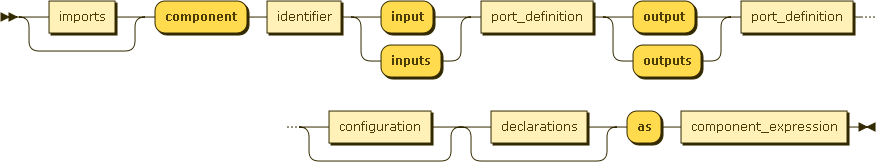
\includegraphics[scale=\DiagramScale,angle=90]{chapters/compiler/diagrams/component}
  \caption{PCL file syntax.}
  \label{fig:pcl-top-level}
\end{figure}

\subsection{Imports}
\begin{figure}[!h]
  \centering
    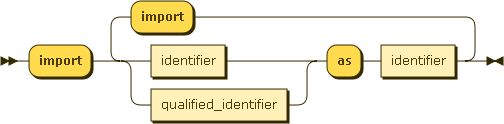
\includegraphics[scale=\DiagramScale]{chapters/compiler/diagrams/imports}
  \caption{\texttt{imports} : Importing PCL files.}
  \label{fig:pcl-imports}
\end{figure}

\subsection{Port Definition}
\begin{figure}[!h]
  \centering
    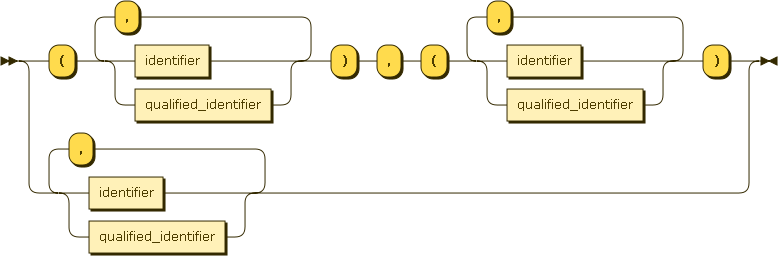
\includegraphics[scale=\DiagramScale,angle=90]{chapters/compiler/diagrams/port_definition}
  \caption{\texttt{port\_definition} : Component port definition.}
  \label{fig:pcl-port-defs}
\end{figure}

\subsection{Configuration}
\begin{figure}[!h]
  \centering
    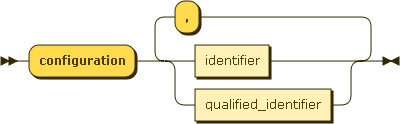
\includegraphics[scale=\DiagramScale]{chapters/compiler/diagrams/configuration}
  \caption{\texttt{configuration} : Component configuraton.}
  \label{fig:pcl-config}
\end{figure}

\subsection{Declarations}
\begin{figure}[!h]
  \centering
    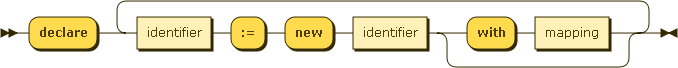
\includegraphics[scale=\DiagramScale]{chapters/compiler/diagrams/declarations}
  \caption{\texttt{declarations} : Imported component construction.}
  \label{fig:pcl-decls}
\end{figure}

\subsection{Definition}
\begin{figure}[!h]
  \centering
    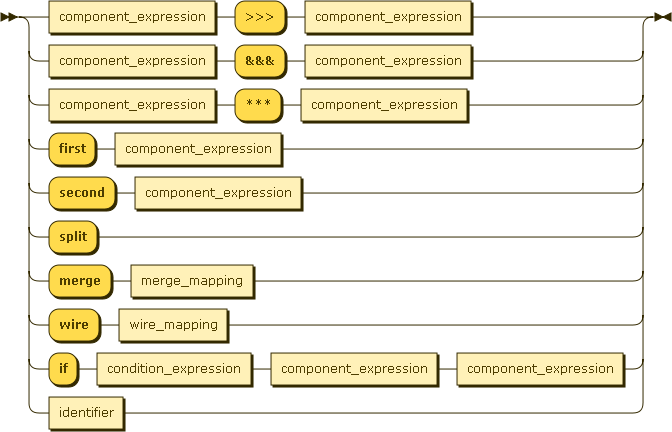
\includegraphics[scale=\DiagramScale,angle=90]{chapters/compiler/diagrams/component_expression}
  \caption{\texttt{component\_expression} : Component defintion.}
  \label{fig:pcl-def}
\end{figure}

\subsection{Merge Mapping}
\begin{figure}[!h]
  \centering
    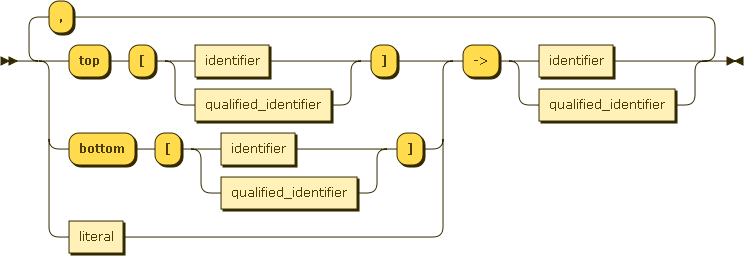
\includegraphics[scale=\DiagramScale,angle=90]{chapters/compiler/diagrams/merge_mapping}
  \caption{\texttt{merge\_mapping} : Merge component mapping.}
  \label{fig:pcl-merge-mapping}
\end{figure}

\subsection{Mapping}
\begin{figure}[!h]
  \centering
    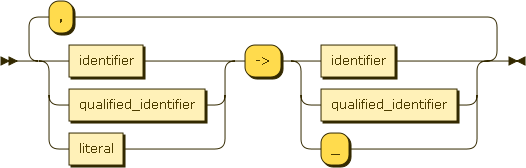
\includegraphics[scale=\DiagramScale]{chapters/compiler/diagrams/mapping}
  \caption{\texttt{mapping} : Mapping.}
  \label{fig:pcl-signal-mapping}
\end{figure}

\subsection{Condition Expression}
\begin{figure}[!h]
  \centering
    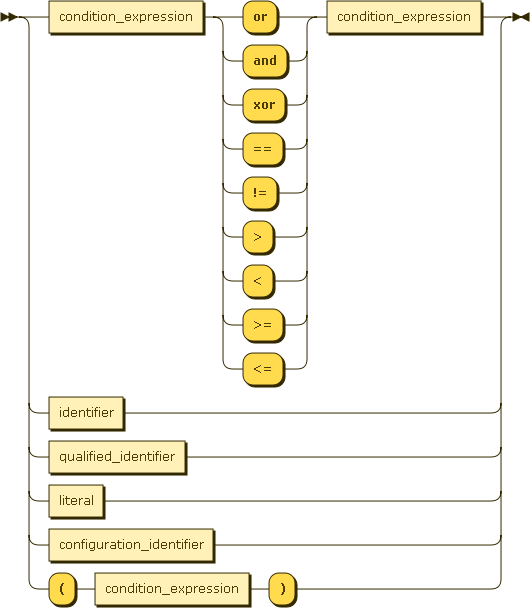
\includegraphics[scale=\DiagramScale]{chapters/compiler/diagrams/condition_expression}
  \caption{\texttt{condition\_expression} : If component's condition expression.}
  \label{fig:pcl-cond-expr}
\end{figure}

\subsection{Configuration Identifier}
\begin{figure}[!h]
  \centering
    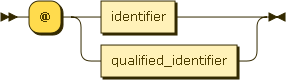
\includegraphics[scale=\DiagramScale]{chapters/compiler/diagrams/configuration_identifier}
  \caption{\texttt{configuration\_identifier} : If component's condition expression configuration identifier.}
  \label{fig:pcl-config-id}
\end{figure}

\subsection{Qualified Identifier}
\begin{figure}[!h]
  \centering
    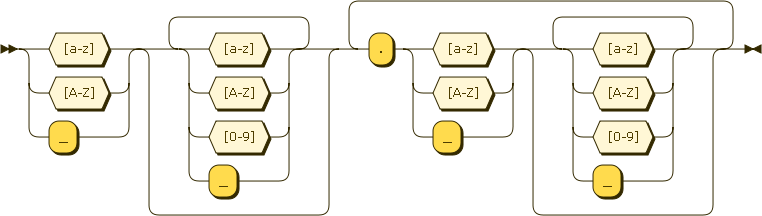
\includegraphics[scale=\DiagramScale,angle=90]{chapters/compiler/diagrams/qualified_identifier}
  \caption{\texttt{qualified\_identifier} : Qualified identifier.}
  \label{fig:pcl-qualified-id}
\end{figure}

\subsection{Identifier}
\begin{figure}[!h]
  \centering
    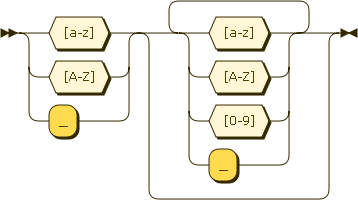
\includegraphics[scale=\DiagramScale]{chapters/compiler/diagrams/identifier}
  \caption{\texttt{identifier} : Identifier.}
  \label{fig:pcl-id}
\end{figure}

\subsection{Literal}
\begin{figure}[!h]
  \centering
    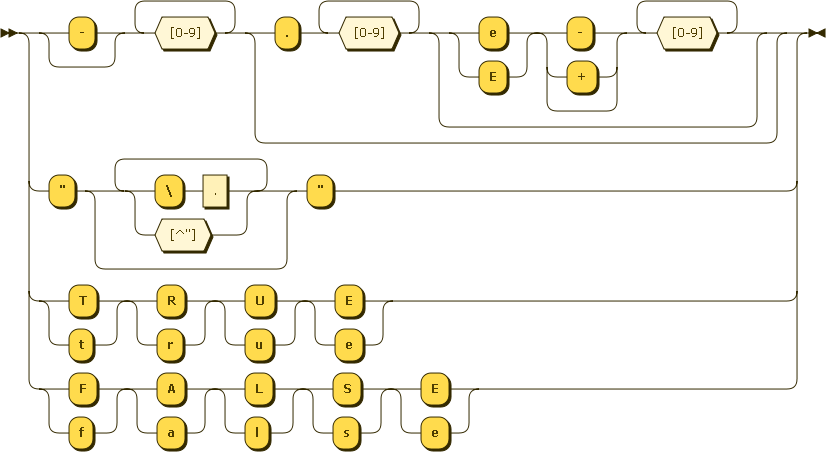
\includegraphics[scale=\DiagramScale,angle=90]{chapters/compiler/diagrams/literal}
  \caption{\texttt{literal} : Literal.}
  \label{fig:pcl-literal}
\end{figure}